\documentclass[11pt,a4paper]{report}
\usepackage[textwidth=37em,vmargin=30mm]{geometry}
\usepackage{calc,xunicode,amsmath,amssymb,paralist,enumitem,tabu,booktabs,datetime2,xeCJK,xeCJKfntef,listings}
\usepackage{tocloft,fancyhdr,tcolorbox,xcolor,graphicx,eso-pic,xltxtra,xelatexemoji}

\newcommand{\envyear}[0]{2025}
\newcommand{\envdatestr}[0]{2025-10-04}
\newcommand{\envfinaldir}[0]{webdb/2025/20251004/final}

\usepackage[hidelinks]{hyperref}
\hypersetup{
    colorlinks=false,
    pdfpagemode=FullScreen,
    pdftitle={Web Digest - \envdatestr}
}

\setlength{\cftbeforechapskip}{10pt}
\renewcommand{\cftchapfont}{\rmfamily\bfseries\large\raggedright}
\setlength{\cftbeforesecskip}{2pt}
\renewcommand{\cftsecfont}{\sffamily\small\raggedright}

\setdefaultleftmargin{2em}{2em}{1em}{1em}{1em}{1em}

\usepackage{xeCJK,xeCJKfntef}
\xeCJKsetup{PunctStyle=plain,RubberPunctSkip=false,CJKglue=\strut\hskip 0pt plus 0.1em minus 0.05em,CJKecglue=\strut\hskip 0.22em plus 0.2em}
\XeTeXlinebreaklocale "zh"
\XeTeXlinebreakskip = 0pt


\setmainfont{Brygada 1918}
\setromanfont{Brygada 1918}
\setsansfont{IBM Plex Sans}
\setmonofont{JetBrains Mono NL}
\setCJKmainfont{Noto Serif CJK SC}
\setCJKromanfont{Noto Serif CJK SC}
\setCJKsansfont{Noto Sans CJK SC}
\setCJKmonofont{Noto Sans CJK SC}

\setlength{\parindent}{0pt}
\setlength{\parskip}{8pt}
\linespread{1.15}

\lstset{
	basicstyle=\ttfamily\footnotesize,
	numbersep=5pt,
	backgroundcolor=\color{black!5},
	showspaces=false,
	showstringspaces=false,
	showtabs=false,
	tabsize=2,
	captionpos=b,
	breaklines=true,
	breakatwhitespace=true,
	breakautoindent=true,
	linewidth=\textwidth
}






\newcommand{\coverpic}[2]{
    % argv: itemurl, authorname
    Cover photo by #2~~(\href{#1}{#1})
}
\newcommand{\makeheader}[0]{
    \begin{titlepage}
        % \newgeometry{hmargin=15mm,tmargin=21mm,bmargin=12mm}
        \begin{center}
            
            \rmfamily\scshape
            \fontspec{BaskervilleF}
            \fontspec{Old Standard}
            \fontsize{59pt}{70pt}\selectfont
            WEB\hfill DIGEST
            
            \vfill
            % \vskip 30pt
            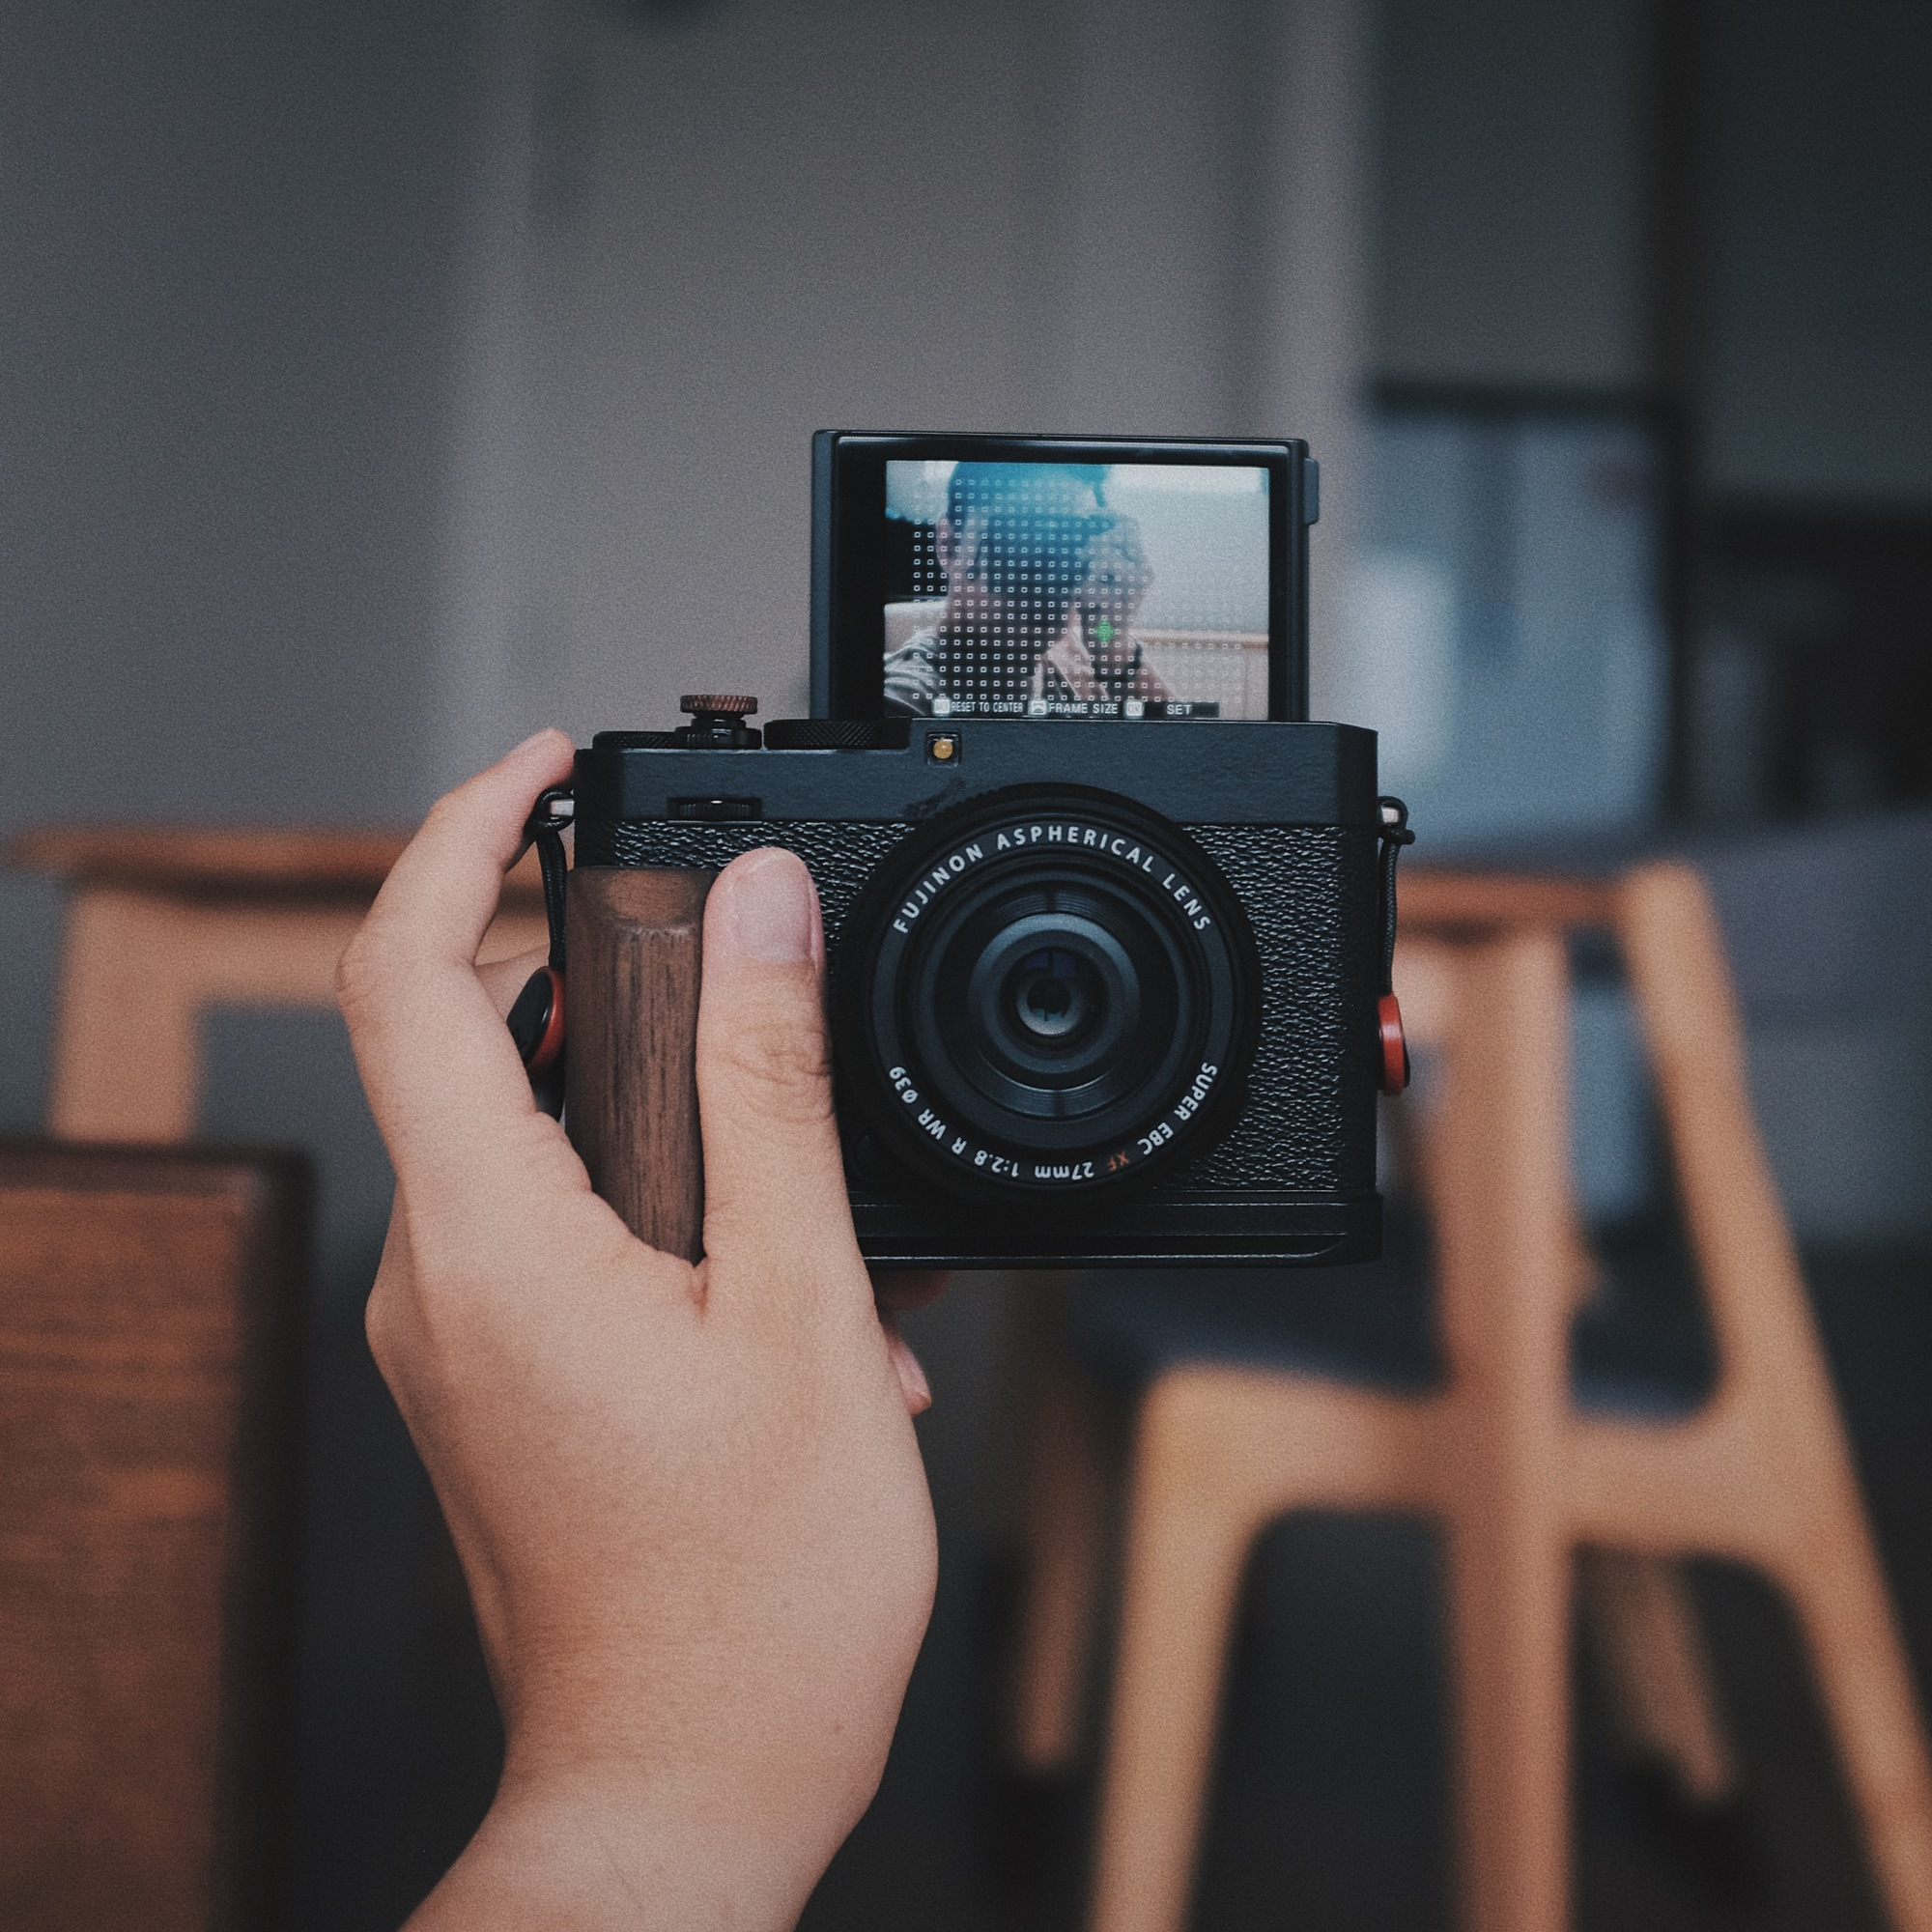
\includegraphics[width=\linewidth]{\envfinaldir/coverpic-prod.jpg}\par
            % \vskip 30pt
            \vfill

            \normalsize\rmfamily\scshape
            \copyright{} The Web Digest Project \hfill\large \envdatestr
        \end{center}
    \end{titlepage}
    % \restoregeometry
}
\newcommand{\simplehref}[1]{%
    \textcolor{blue!80!green}{\href{#1}{#1}}%
}
\renewcommand{\contentsname}{\center\Huge\sffamily\bfseries Contents\par\vskip 20pt}
\newcounter{ipartcounter}
\setcounter{ipartcounter}{0}
\newcommand{\ipart}[1]{
    % \vskip 20pt
    \clearpage
    \stepcounter{ipartcounter}
    \phantomsection
    \addcontentsline{toc}{chapter}{#1}
    % \begin{center}
    %     \Huge
    %     \sffamily\bfseries
    %     #1
    % \end{center}
    % \vskip 20pt plus 7pt
}
\newcounter{ichaptercounter}
\setcounter{ichaptercounter}{0}
\newcommand{\ichapter}[1]{
    % \vskip 20pt
    \clearpage
    \stepcounter{ichaptercounter}
    \phantomsection
    \addcontentsline{toc}{section}{\numberline{\arabic{ichaptercounter}}#1}
    \begin{center}
        \Huge
        \sffamily\bfseries
        #1
    \end{center}
    \vskip 20pt plus 7pt
}
\newcommand{\entrytitlefont}[1]{\subsection*{\raggedright\Large\sffamily\bfseries#1}}
\newcommand{\entryitemGeneric}[2]{
    % argv: title, url
    \parbox{\linewidth}{
        \entrytitlefont{#1}\par\vskip 5pt
        \footnotesize\ttfamily\mdseries
        \simplehref{#2}
    }\vskip 11pt plus 11pt minus 1pt
}
\newcommand{\entryitemGithub}[3]{
    % argv: title, url, desc
    \parbox{\linewidth}{
        \entrytitlefont{#1}\par\vskip 5pt
        \footnotesize\ttfamily\mdseries
        \simplehref{#2}\par\vskip 5pt
        \small\rmfamily\mdseries#3
    }\vskip 11pt plus 11pt minus 1pt
}
\newcommand{\entryitemAp}[3]{
    % argv: title, url, desc
    \parbox{\linewidth}{
        \entrytitlefont{#1}\par\vskip 5pt
        \footnotesize\ttfamily\mdseries
        \simplehref{#2}\par\vskip 5pt
        \small\rmfamily\mdseries#3
    }\vskip 11pt plus 11pt minus 1pt
}
\newcommand{\entryitemHackernews}[3]{
    % argv: title, hnurl, rawurl
    % \parbox{\linewidth}{
    %     \entrytitlefont{#1}\par\vskip 5pt
    %     \footnotesize\ttfamily\mdseries
    %     \simplehref{#3}\par
    %     \textcolor{black!50}{\href{#2}{#2}}
    % }\vskip 11pt plus 11pt minus 1pt
    \begin{minipage}{\linewidth}
            \entrytitlefont{#1}\par\vskip 5pt
            \footnotesize\ttfamily\mdseries
            \simplehref{#3}\par
            \textcolor{black!50}{\href{#2}{#2}}
    \end{minipage}\par\vskip 11pt plus 11pt minus 1pt
}







\begin{document}

\makeheader

\tableofcontents\clearpage




\ipart{Developers}
\ichapter{Hacker News}
\entryitemTwoLinks{Offline card payments should be possible no later than 1 July 2026}{https://news.ycombinator.com/item?id=45467500}{https://www.riksbank.se/en-gb/press-and-published/notices-and-press-releases/press-releases/2025/offline-card-payments-should-be-possible-no-later-than-1-july-2026/}

\entryitemTwoLinks{PEP 810 – Explicit lazy imports}{https://news.ycombinator.com/item?id=45466086}{https://pep-previews--4622.org.readthedocs.build/pep-0810/}

\entryitemTwoLinks{ICE Wants to Build Out a 24/7 Social Media Surveillance Team}{https://news.ycombinator.com/item?id=45465964}{https://www.wired.com/story/ice-social-media-surveillance-24-7-contract/}

\entryitemTwoLinks{Ants trapped in a Soviet nuclear bunker survived for years}{https://news.ycombinator.com/item?id=45465091}{https://www.sciencealert.com/ants-trapped-in-an-old-soviet-nuclear-bunker-survived-for-years-by-turning-on-their-own}

\entryitemTwoLinks{The collapse of the econ PhD job market}{https://news.ycombinator.com/item?id=45464984}{https://www.chrisbrunet.com/p/the-collapse-of-the-econ-phd-job}

\entryitemTwoLinks{Germany must stand firmly against client-side scanning in Chat Control [pdf]}{https://news.ycombinator.com/item?id=45464921}{https://signal.org/blog/pdfs/germany-chat-control.pdf}

\entryitemTwoLinks{OpenAI Is Just Another Boring, Desperate AI Startup}{https://news.ycombinator.com/item?id=45464849}{https://www.wheresyoured.at/sora2-openai/}

\entryitemTwoLinks{Cancelling async Rust}{https://news.ycombinator.com/item?id=45464632}{https://sunshowers.io/posts/cancelling-async-rust/}

\entryitemTwoLinks{Anduril and Palantir battlefield communication system has flaws, Army memo says}{https://news.ycombinator.com/item?id=45464269}{https://www.cnbc.com/2025/10/03/anduril-palantir-ngc2-deep-flaws-army.html}

\entryitemTwoLinks{Social anxiety isn't about being liked}{https://news.ycombinator.com/item?id=45463656}{https://chrislakin.blog/p/social-anxiety}

\entryitemTwoLinks{Microsoft CTO says he wants to swap most AMD and Nvidia GPUs for homemade chips}{https://news.ycombinator.com/item?id=45463642}{https://www.cnbc.com/2025/10/01/microsoft-wants-to-mainly-use-its-own-ai-chips-in-the-future.html}

\entryitemTwoLinks{I turned the Lego Game Boy into a working Game Boy}{https://news.ycombinator.com/item?id=45463319}{https://blog.nataliethenerd.com/i-turned-the-lego-game-boy-into-a-working-game-boy-part-1/}

\entryitemTwoLinks{Webbol: A minimal static web server written in COBOL}{https://news.ycombinator.com/item?id=45463251}{https://github.com/jmsdnns/webbol}

\entryitemTwoLinks{The Faroes}{https://news.ycombinator.com/item?id=45462297}{https://photoblog.nk412.com/Faroe2025/Faroes/n-cPCNFr}

\entryitemTwoLinks{Niri – A scrollable-tiling Wayland compositor}{https://news.ycombinator.com/item?id=45461500}{https://github.com/YaLTeR/niri}

\entryitemTwoLinks{In Praise of RSS and Controlled Feeds of Information}{https://news.ycombinator.com/item?id=45459233}{https://blog.burkert.me/posts/in\_praise\_of\_syndication/}

\entryitemTwoLinks{Fp8 runs ~100 tflops faster when the kernel name has "cutlass" in it}{https://news.ycombinator.com/item?id=45458948}{https://github.com/triton-lang/triton/pull/7298}

\entryitemTwoLinks{Digital ID – The New Chains of Capitalist Surveillance}{https://news.ycombinator.com/item?id=45458909}{https://theslowburningfuse.wordpress.com/2025/09/26/digital-id-the-new-chains-of-capitalist-surveillance/}

\entryitemTwoLinks{Blender 4.5 LTS}{https://news.ycombinator.com/item?id=45458791}{https://lwn.net/Articles/1036262/}

\entryitemTwoLinks{Stdlib: A library of frameworks, templates, and guides for technical leadership}{https://news.ycombinator.com/item?id=45458249}{https://debuggingleadership.com/stdlib}\ichapter{Phoronix}
\entryitemGeneric{\hskip 0pt{}Linux 6.18 Will Be A Big Improvement For Servers Encountering DDoS Attacks}{https://www.phoronix.com/news/Linux-6.18-DDoS-Improvement}

\entryitemGeneric{\hskip 0pt{}Linux 6.18 Lands Compress-Offload API For Opus Audio Codec}{https://www.phoronix.com/news/Linux-6.18-Sound}

\entryitemGeneric{\hskip 0pt{}Rusticl Performance For AMD Strix Halo Against ROCm OpenCL}{https://www.phoronix.com/review/rocm-7-rusticl-opencl}

\entryitemGeneric{\hskip 0pt{}Linux 6.18 Device Tree Prepares For Arm C1 Nano / Pro / Platinum / Ultra CPUs}{https://www.phoronix.com/news/Linux-6.18-Device-Tree}

\entryitemGeneric{\hskip 0pt{}Intel NPU Linux Driver 1.24 Released}{https://www.phoronix.com/news/Intel-NPU-Linux-Driver-1.24}

\entryitemGeneric{\hskip 0pt{}Ubuntu 25.10 Ready With "Stubble" For Better ARM64 Experience}{https://www.phoronix.com/news/Ubuntu-25.10-Stubble-Ready}

\entryitemGeneric{\hskip 0pt{}Qualcomm Iris Driver Adds H.264/H.265 Encode, Sadly No AMD ISP4 Driver For Linux 6.18}{https://www.phoronix.com/news/Linux-6.18-Media-Subsystem}

\entryitemGeneric{\hskip 0pt{}Free Software Foundation Names New President}{https://www.phoronix.com/news/FSF-New-President-2025}

\entryitemGeneric{\hskip 0pt{}Linux 6.18 Non-MM Pull Request: "A Mere 150x Speedup Was Measured..."}{https://www.phoronix.com/news/Linux-6.18-Non-MM-PR}


\ipart{Developers~~~~(zh-Hans)}
\ichapter{Solidot}
\entryitemGeneric{\hskip 0pt{}英特尔与 AMD 磋商代工芯片}{https://www.solidot.org/story?sid=82471}

\entryitemGeneric{\hskip 0pt{}印度高等法院要求医生书写清晰的处方}{https://www.solidot.org/story?sid=82470}

\entryitemGeneric{\hskip 0pt{}黑客声称入侵了 Red Hat 的 GitHub 代码库}{https://www.solidot.org/story?sid=82469}

\entryitemGeneric{\hskip 0pt{}千禧一代癌症发病率在上升}{https://www.solidot.org/story?sid=82468}

\entryitemGeneric{\hskip 0pt{}城市空气检测出致病性酵母菌株}{https://www.solidot.org/story?sid=82467}

\entryitemGeneric{\hskip 0pt{}珍·古道尔去世,享年 91 岁}{https://www.solidot.org/story?sid=82466}

\entryitemGeneric{\hskip 0pt{}Kindle Scribe 加入 AI 驱动的笔记本功能}{https://www.solidot.org/story?sid=82465}

\entryitemGeneric{\hskip 0pt{}Imgur 屏蔽英国用户访问}{https://www.solidot.org/story?sid=82464}

\entryitemGeneric{\hskip 0pt{}微软宣布 Windows 11 v25H2 GA}{https://www.solidot.org/story?sid=82463}

\entryitemGeneric{\hskip 0pt{}Cloudflare 赞助 Ladybird 浏览器引擎项目}{https://www.solidot.org/story?sid=82462}\ichapter{V2EX}
\entryitemGeneric{\hskip 0pt{}[问与答] upnote 用户有吗?我的 upnote 无法联网了}{https://www.v2ex.com/t/1163303}

\entryitemGeneric{\hskip 0pt{}[开源软件] 想做这个一个开源的导航页面}{https://www.v2ex.com/t/1163302}

\entryitemGeneric{\hskip 0pt{}[Apple] 2025 年了 iPhone 照片还有什么非 iCloud 的备份方案吗?}{https://www.v2ex.com/t/1163301}

\entryitemGeneric{\hskip 0pt{}[推广] 做了一款实时 AI 换脸软件,自认为业界最好用(没有之一), 付费率高的很,就是规模上不去!有没有大佬指点一下}{https://www.v2ex.com/t/1163300}

\entryitemGeneric{\hskip 0pt{}[NAS] 垃圾阿三 Windows,局域网 win7 共享文件夹, win10 搜不到}{https://www.v2ex.com/t/1163299}

\entryitemGeneric{\hskip 0pt{}[北京] 在北京花 4500 租房,很奢侈么?}{https://www.v2ex.com/t/1163297}

\entryitemGeneric{\hskip 0pt{}[macOS] spotlight 用英文名搜索应用不走索引了?}{https://www.v2ex.com/t/1163296}

\entryitemGeneric{\hskip 0pt{}[Apple] 最近有 v 友成功在苹果官网买礼品卡成功了吗?求指导}{https://www.v2ex.com/t/1163295}

\entryitemGeneric{\hskip 0pt{}[Apple] 求推荐小米的金沙江充电宝平替}{https://www.v2ex.com/t/1163294}

\entryitemGeneric{\hskip 0pt{}[分享创造] [工具发布] AI Figure Generator — 3D 手办生成器}{https://www.v2ex.com/t/1163293}

\entryitemGeneric{\hskip 0pt{}[随想] 快三十了,聊聊一千六海拔瘫在床上的身体}{https://www.v2ex.com/t/1163292}

\entryitemGeneric{\hskip 0pt{}[问与答] 网工进来,关于 pathping 速度疑问}{https://www.v2ex.com/t/1163291}

\entryitemGeneric{\hskip 0pt{}[问与答] 为啥 ChatGPT 和 Claude 不能好好显示历史记录时间?直接显示具体年月日时分秒不行吗?}{https://www.v2ex.com/t/1163287}

\entryitemGeneric{\hskip 0pt{}[Android] 安卓原生开发,怎么利用 Claude 等 AI 辅助编程?}{https://www.v2ex.com/t/1163286}

\entryitemGeneric{\hskip 0pt{}[macOS] macOS 备忘录关闭并重新打开后,才能同步至 iPhone}{https://www.v2ex.com/t/1163284}

\entryitemGeneric{\hskip 0pt{}[分享创造] 做了个 sora 2 生成网站,有需要的朋友可以过来体验}{https://www.v2ex.com/t/1163283}

\entryitemGeneric{\hskip 0pt{}[问与答] 如何提高 claude code 指令遵循,经常让他做 A,帮我做了 ABC……}{https://www.v2ex.com/t/1163282}

\entryitemGeneric{\hskip 0pt{}[程序员] 小白有个问题,有没有方法把一套程序(如 discuz)喂给 AI 呢?}{https://www.v2ex.com/t/1163281}

\entryitemGeneric{\hskip 0pt{}[酷工作] [远程全职] 日本 SaaS 上市公司:全栈、后端、DevOps}{https://www.v2ex.com/t/1163280}

\entryitemGeneric{\hskip 0pt{}[宽带症候群] 如何判断分流规则是否导致国内网站风控?}{https://www.v2ex.com/t/1163276}

\entryitemGeneric{\hskip 0pt{}[问与答] 有没有什么工具可以统计 C++项目里标识符的使用情况?}{https://www.v2ex.com/t/1163273}

\entryitemGeneric{\hskip 0pt{}[Apple] 有没有觉得 iOS 现在删除 App 好繁琐}{https://www.v2ex.com/t/1163272}

\entryitemGeneric{\hskip 0pt{}[优惠信息] 腾讯云续费拼团}{https://www.v2ex.com/t/1163271}

\entryitemGeneric{\hskip 0pt{}[Windows] OOBE(初始设置)为 欧盟国家 的 Windows 11 IoT LTSC,可以官方卸载 edge 浏览器吗?}{https://www.v2ex.com/t/1163270}

\entryitemGeneric{\hskip 0pt{}[程序员] 通义万相 2.5 已经发布了,和 sora2 的区别大吗}{https://www.v2ex.com/t/1163269}

\entryitemGeneric{\hskip 0pt{}[加密货币] 助记词分片工具}{https://www.v2ex.com/t/1163265}

\entryitemGeneric{\hskip 0pt{}[Linux] 微信 for Linux 更新到 4.1.0 了}{https://www.v2ex.com/t/1163264}

\entryitemGeneric{\hskip 0pt{}[问与答] MX Master 3 侧键总成哪里修?}{https://www.v2ex.com/t/1163263}

\entryitemGeneric{\hskip 0pt{}[iPad] 官网 2024 iPad Pro 开始缺货了}{https://www.v2ex.com/t/1163261}

\entryitemGeneric{\hskip 0pt{}[分享创造] 试出了用 AI 把静态图片批量快速转成动态 GIF 的方法}{https://www.v2ex.com/t/1163260}

\entryitemGeneric{\hskip 0pt{}[问与答] 免费的闲鱼违禁词检测工具,可检测图片}{https://www.v2ex.com/t/1163259}

\entryitemGeneric{\hskip 0pt{}[广州] 跟父亲的关系,可能如风筝一样}{https://www.v2ex.com/t/1163258}

\entryitemGeneric{\hskip 0pt{}[生活] 杭州烘培甜点行业求助}{https://www.v2ex.com/t/1163257}

\entryitemGeneric{\hskip 0pt{}[宽带症候群] 国庆回老家突然发现路由器下发了恶意的 dns}{https://www.v2ex.com/t/1163254}

\entryitemGeneric{\hskip 0pt{}[分享创造] 因为经常测试修改 zsh 等配置文件后忘了怎么改回原样,所以写了一个简洁的文件自动快照的应用,现在已经可以在 testflight 下载了}{https://www.v2ex.com/t/1163252}

\entryitemGeneric{\hskip 0pt{}[分享创造] 用 cursor 一晚上搓出来的网站!旅游必须要有它!大幅提高效率}{https://www.v2ex.com/t/1163251}

\entryitemGeneric{\hskip 0pt{}[Android] 推荐个安卓机,用来备用的}{https://www.v2ex.com/t/1163250}

\entryitemGeneric{\hskip 0pt{}[分享发现] 四部门:规范酒店电视服务 加强酒店电视管理}{https://www.v2ex.com/t/1163249}

\entryitemGeneric{\hskip 0pt{}[生活] 焦虑症日记:十一也崩溃。}{https://www.v2ex.com/t/1163248}

\entryitemGeneric{\hskip 0pt{}[深圳] 在深圳的朋友国庆期间都是怎么过的}{https://www.v2ex.com/t/1163246}

\entryitemGeneric{\hskip 0pt{}[分享创造] 100 个着陆页实验之二}{https://www.v2ex.com/t/1163245}

\entryitemGeneric{\hskip 0pt{}[分享创造] Sora2 网站肛好了,并且支持自动「去除水印」}{https://www.v2ex.com/t/1163241}

\entryitemGeneric{\hskip 0pt{}[问与答] 有没有虚拟卡商?用来开 0 刀 team 的。要求稳定一点,量多。有的话加 v:thisiseasytosearch}{https://www.v2ex.com/t/1163240}

\entryitemGeneric{\hskip 0pt{}[Apple] iPhone 17 pro max 充电还挺快的,洗个澡就差不多了}{https://www.v2ex.com/t/1163238}

\entryitemGeneric{\hskip 0pt{}[程序员] 国庆期间我的一个 2 年的 claude 账号和一个 1 一个月的 claude 相继被封}{https://www.v2ex.com/t/1163237}

\entryitemGeneric{\hskip 0pt{}[分享创造] 开源了个 database 版本的 ClaudeCodeCLI - DBSage}{https://www.v2ex.com/t/1163235}

\entryitemGeneric{\hskip 0pt{}[Terminal] 大家碰到了 ms terminal 的行缓冲区错乱的问题么?}{https://www.v2ex.com/t/1163234}

\entryitemGeneric{\hskip 0pt{}[程序员] 抛开性价比这个选项,你认为目前写代码最强模型是?}{https://www.v2ex.com/t/1163230}

\entryitemGeneric{\hskip 0pt{}[问与答] 为什么小米音箱的唤醒词这么多年了还是「小爱同学」而不能精简下?}{https://www.v2ex.com/t/1163229}

\entryitemGeneric{\hskip 0pt{}[分享发现] YouTube Premium 新政策,如何防止被停?}{https://www.v2ex.com/t/1163228}


\ipart{Generic News}







\clearpage
\leavevmode\vfill
\footnotesize

Copyright \copyright{} 2023-2025 Neruthes and other contributors.

This document is published with CC BY-NC-ND 4.0 license.

The entries listed in this newsletter may be copyrighted by their respective creators.

This newsletter is generated by the Web Digest project.

The newsletters are also delivered via Telegram channel \CJKunderline{\href{https://t.me/webdigestchannel}{https://t.me/webdigestchannel}}.\\
RSS feed is available at \CJKunderline{\href{https://webdigest.pages.dev/rss.xml}{https://webdigest.pages.dev/rss.xml}}.

This newsletter is available in PDF at
\CJKunderline{\href{https://webdigest.pages.dev/}{https://webdigest.pages.dev/}}.

The source code being used to generate this newsletter is available at\\
\CJKunderline{\href{https://github.com/neruthes/webdigest}{https://github.com/neruthes/webdigest}}.

This newsletter is also available in
\CJKunderline{\href{http://webdigest.pages.dev/readhtml/\envyear/WebDigest-20251004.html}{HTML}} and
\CJKunderline{\href{https://github.com/neruthes/webdigest/blob/master/markdown/\envyear/WebDigest-20251004.md}{Markdown}}.


\coverpic{https://unsplash.com/photos/woman-posing-on-a-bridge-with-gondola-in-venice-JULr9w9FEHk}{Karsten Winegeart}


\end{document}
